%Skal være under object recognition section
\subsection{OpenCV}
\begin{frame}[fragile]{\insertsection}
  \tableofcontents[currentsubsection]
\end{frame}

\begin{frame}[fragile]{\insertsection}{\insertsubsection -Template Matching}
	\begin{itemize}
		\item Hvad er OpenCV?
			\item Template Matching: matching\_\ method(cimg, templ, CV\_\ TM\_\ CCOEFF\_\ NORMED);
	\end{itemize}
	\begin{figure}
		\begin{minipage}{0.20\textwidth}
			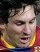
\includegraphics[scale=1]{pictures/messi_face.jpg}
		\end{minipage}
		\begin{minipage}{0.75\textwidth}
			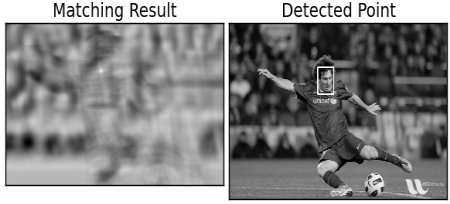
\includegraphics[width=\textwidth]{pictures/template_ccorrn_4.jpg}				
		\end{minipage}
		\caption{http://docs.opencv.org/3.1.0/d4/dc6/tutorial\_\ py\_\ template\_\ matching.html\#\ gsc.tab=0}
	\end{figure}
\end{frame}
%http://docs.opencv.org/3.1.0/d4/dc6/tutorial_py_template_matching.html#gsc.tab=0

\begin{frame}[fragile]{\insertsection}{fordele/ulemper ved Template Matching}
	\begin{figure}[t]
		\begin{minipage}[t]{.45\textwidth}
			Fordele:
			\begin{itemize}
				\item Simpel metode
				\item Bred anvendelighed
			\end{itemize}
		\end{minipage}
		\begin{minipage}[t]{.45\textwidth}
			Ulemper:			
			\begin{itemize}
				\item Naiv
				\item Ikke skalerings invariant
				\item Ikke rotations invariant
			\end{itemize}
		\end{minipage}
	\end{figure}
\end{frame}

\begin{frame}[fragile]{\insertsection}{\insertsubsection -Anden metode}

	\begin{itemize}
		\item Konvertering fra RGB til HSV
		\begin{figure}
			\begin{minipage}{.9\textwidth}
				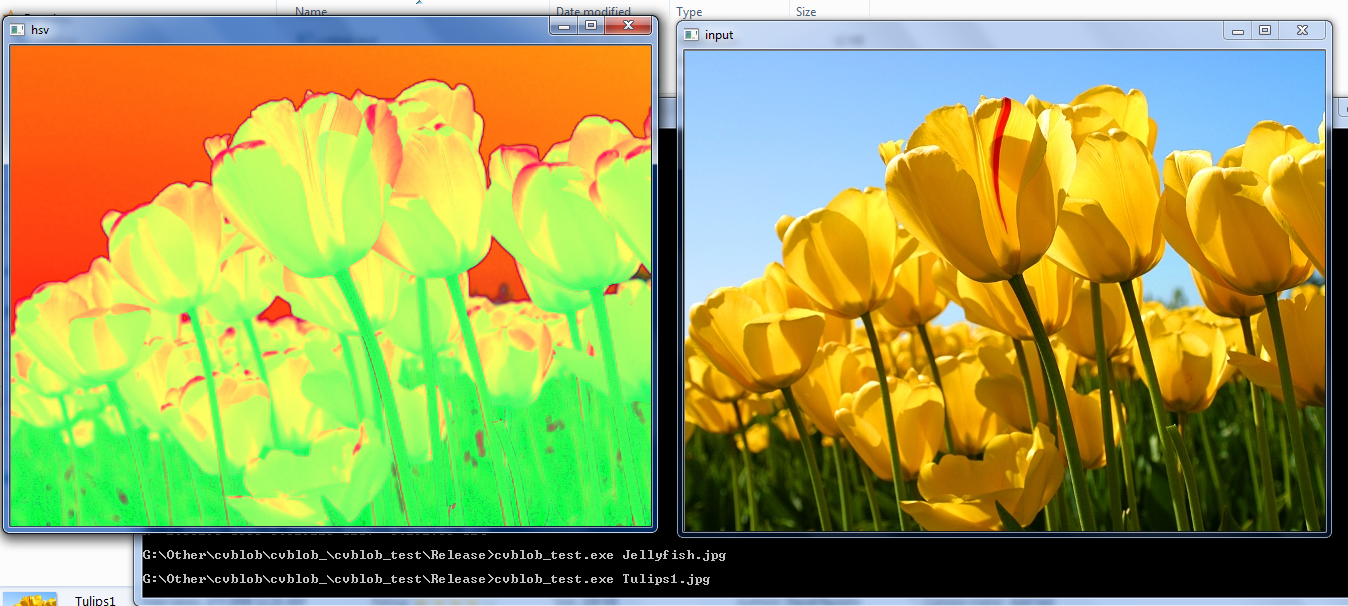
\includegraphics[width=\textwidth]{pictures/rgbtohsv.png}
				\caption{http://www.technolabsz.com/2012/08/how-to-convert-rgb-to-hsv-using-opencv.html}
			\end{minipage}
		\end{figure}
	\end{itemize}
\end{frame}
%http://www.technolabsz.com/2012/08/how-to-convert-rgb-to-hsv-using-opencv.html

\begin{frame}[fragile]{\insertsection}{\insertsubsection -Anden metode}
	\begin{itemize}
		\item Fra RGB til HSV til binær repræsentation
		\begin{figure}
			\begin{minipage}{.9\textwidth}
				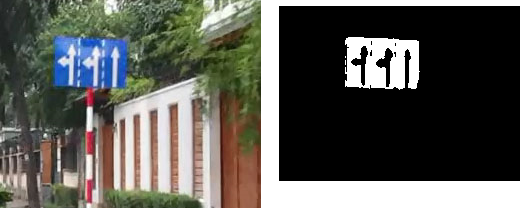
\includegraphics[width=\textwidth]{pictures/rgbhsv.png}
				\caption{http://stackoverflow.com/questions/17063042/why-do-we-convert-from-rgb-to-hsv}
			\end{minipage}
		\end{figure}
	\end{itemize}
\end{frame}
%http://stackoverflow.com/questions/17063042/why-do-we-convert-from-rgb-to-hsv

\begin{frame}[fragile]{\insertsection}{\insertsubsection -Anden metode}
	\begin{itemize}
		\item Thresholding med dilatation og erosion  
		\begin{figure}
			\begin{minipage}{.30\textwidth}
				
\includegraphics[width=.7\textwidth]{pictures/i_norm.png}
				\caption{Normalt billede}
			\end{minipage}
			\begin{minipage}{.30\textwidth}
				
\includegraphics[width=.7\textwidth]{pictures/i_dilated.png}
				\caption{Dilateret billede}
			\end{minipage}
			\begin{minipage}{.30\textwidth}
				
\includegraphics[width=.7\textwidth]{pictures/i_eroded.png}
				\caption{Eroderet billede}
			\end{minipage}
		\end{figure}
	\end{itemize}
\end{frame}
%http://docs.opencv.org/2.4/doc/tutorials/imgproc/erosion_dilatation/erosion_dilatation.html

\begin{frame}[fragile]{\insertsection}{\insertsubsection -Anden metode}
	\begin{figure}
		\begin{minipage}{.9\textwidth}
			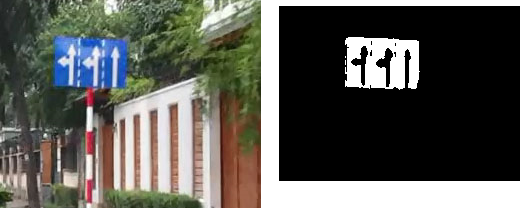
\includegraphics[width=\textwidth]{pictures/rgbhsv.png}
			\caption{http://stackoverflow.com/questions/17063042/why-do-we-convert-from-rgb-to-hsv}
		\end{minipage}
	\end{figure}
\end{frame}
%http://stackoverflow.com/questions/17063042/why-do-we-convert-from-rgb-to-hsv